\section{The experiments}
\stlabel{experiments}

We have carried out experiments based on three rule systems with varying
characteristics.

\begin{description}
\item[le] A leader election protocol. In this case there is a fixed number of
  nodes representing network nodes and a varying number of nodes
  representing messages. The number of nodes is an upper limit on the number of
  messages. This case study has been used for the GraBaTs 2009 tool
  contest (see \url{http://is.tm.tue.nl/staff/pvgorp/events/grabats2009}).

\item[unflagged-platoon] A protocol for forming car platoons. In this model
  there is always a fixed number of nodes. The behaviour shows extensive
  symmetries; reduction modulo isomorphism shrinks the state space by many
  orders of magnitude. This case study has been used for the Transformation
  Tool Contest 2010 (see \url{http://planet-research20.org/ttc2010}).

\item[append] A model of list appenders that concurrently add a value to the
  same list. In this case the number of nodes grows in each step. The maximal
  number of nodes equals the number of appenders plus 1 times the number of
  elements in the list. There is hardly any nontrivial isomorphism in the
  transition system.
\end{description}
%
The experiments have been performed on a cluster consisting of 8 compute nodes
with 4 dual Intel E5520 CPUs each and 24GB RAM, for a total of 8 cores per
compute node and 64 cores in total.  \GROOVE 4.0.1 has been used with a Sun
Java 1.6.0 64-bit VM with a maximum of 2GB of memory for each core. For
computing canonical forms we used \BLISS 0.50. We used \LTSMIN 1.5, with an
added dataflow module to facilitate the communication between \LTSMIN and
\GROOVE. For all experiments, the combined system was given a time limit of 4
hours. The state vector size for the first two cases was chosen such that
$n\geq k+5$, hence no slot needs to encode the edges of more than one node;
however, this is not the case for the third case.

We have compared the performance of the distributed setting with the default,
sequential implementation of \GROOVE (without computation of canonical forms), 
running on the same machine but with a
memory upper bound of 20GB. For the leader election with start state
\texttt{start-7p} a different machine with 60GB of memory has been used,
because with 20GB of memory the result could not be calculated.

Where there are no values in the table or figures of this section, either the
time limit of 4 hours was exceeded or there was not enough memory.

\begin{table}
\caption{Results for the largest start graphs where both \GROOVE (sequential)
and \LTSMIN (1, 8 and 64 cores) were able to generate the state-space. The memory usage shown is the average per core. The last column shows the number of elements in the global leaf database for \LTSMIN.}
\tlabel{results}
\begin{center}
\begin{tabular}{|l|r|c|r|r@{\;}r|r@{\;}r|}
\hline
\bf Grammar/ & \bf States/ &  &  & \bf Time &  & \bf Mem &  \\
\bf Start State & \bf Transitions & \bf Tool & \bf Cores & \bf (s) & \bf Speedup & \bf (MB) & \bf Leaf db \\
\hline\hline
\textbf{le} & 3.724.544 & \multicolumn{2}{|l|}{\GROOVE} & 5.128 &  & 2.751 &  \\
\cline{3-8}
start-7p & 16.956.727 & \LTSMIN & 1 & -- & -- & -- &  \\
\cline{4-8}
 &  &  & 8 & 2.005 & 2,6 & 52 & \\
\cline{4-8}
 &  &  & 64 & 307 & 16,7 & 52 & 1.819  \\
\hline\hline
\textbf{unflagged-platoon} & 1.580.449 & \multicolumn{2}{|l|}{\GROOVE} & 1.016 &  & 1.259 &  \\
\cline{3-8}
start-10 & 10.200.436 & \LTSMIN & 1 & 6.621 & 0,2 & 120 &  \\
\cline{4-8}
 &  &  & 8 & 889 & 1,1 & 54 & \\
\cline{4-8}
 &  &  & 64 & 156 & 6,5 & 54 & 8.534  \\
\hline\hline
\textbf{append} & 261.460 & \multicolumn{2}{|l|}{\GROOVE} & 202 &  & 372 &  \\
\cline{3-8}
append-4-list-8 & 969.977 & \LTSMIN & 1 & 3.285 & 0,1 & 99 &  \\
\cline{4-8}
 &  &  & 8 & 352 & 0,6 & 76 & \\
\cline{4-8}
 &  &  & 64 & 92 & 2,2 & 70 & 69.147  \\
\hline
\end{tabular}
\end{center}
\end{table}

\medskip\noindent\textbf{Global results.}\enspace
%
\tref{results} shows some global results for the three cases, using the largest
start graphs for which the sequential setting could compute the entire state
space. We can observe that with 8 cores, the distributed setting starts to
outperform the sequential, and also that the speedup increase from 1 to 8 cores
and from 8 to 64 cores is sizeable, though below the optimal value of 8.
Furthermore, the leaf database of the append rule system grows much larger than
for the others, despite the fact that the state space is much smaller. This is
a consequence of the fact that the graph size outgrows the vector size for this
case.

\begin{figure}[tph]
\addtocounter{figure}{-1}
\centering
\subfloat[Number of states, transitions and leaf values.]{\flabel{size:unflagged-platoon}
    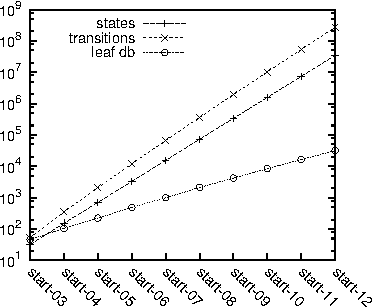
\includegraphics[width=2.7in]{results/graphs/size_unflagged-platoon.pdf}
 }
\quad
\subfloat[Memory usage for \GROOVE and \LTSMIN (per core).]{\flabel{mem:unflagged-platoon}
   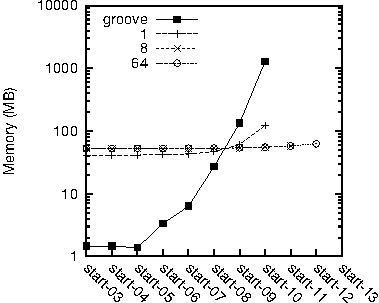
\includegraphics[width=2.7in]{results/graphs/mem_unflagged-platoon.pdf}
 }
\\
  \subfloat[Execution time.]{\flabel{results:unflagged-platoon}
    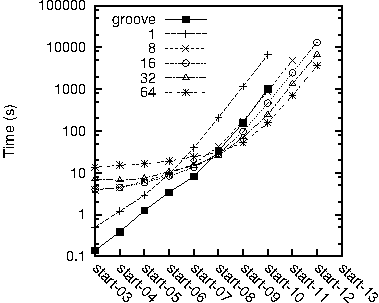
\includegraphics[width=2.7in]{results/graphs/results_unflagged-platoon.pdf}
  }
\quad
 \subfloat[Speedup compared to \GROOVE.]{\flabel{speedup:unflagged-platoon}
    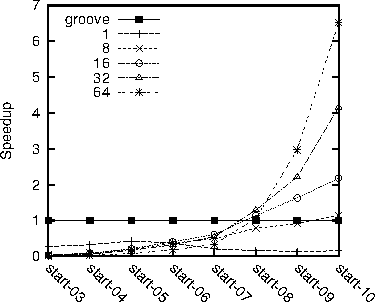
\includegraphics[width=2.7in]{results/graphs/results_unflagged-platoon_speedup.pdf}
  }
\addtocounter{figure}{1}
\caption{Figures for the car platooning case for different start states.}
\flabel{results-unflagged-platoon}
\end{figure}

\medskip\noindent\textbf{Time and memory distributions.}\enspace
%
For the car platooning case, more detailed results are shown in Figures
\ref{fig:results-unflagged-platoon}
and~\ref{fig:results-unflagged-platoon-stacked}. First of all,
\fref{size:unflagged-platoon} shows that even though the size of the problem
grows exponentially, the number of elements of the leaf value database of
\LTSMIN does not. This is also reflected by the per-core memory usage of
\LTSMIN (\fref{mem:unflagged-platoon}), which seems hardly to grow, in contrast
to the more than exponentially growing memory usage of \GROOVE.

Figures \ref{fig:results:unflagged-platoon}
and~\ref{fig:speedup:unflagged-platoon} show the execution time respectively
the speedup of \LTSMIN with different numbers of cores compared to \GROOVE. The
execution time of \LTSMIN with one core is much worse than \GROOVE, but the
speedup is growing fast. For the start states with 11 and 12 cars, \GROOVE
cannot generate the state-space within 4 hours, but \LTSMIN with 8 respectively
16 or more cores can.

\begin{figure}[th]
\addtocounter{figure}{-1}
\newcommand{\inputresult}[1]{\parbox{2.7in}{
   \includegraphics[width=2.3in]{results/graphs/#1.pdf}}
}
\centering
%\subfloat[Execution times for \texttt{start-08}.]{
%  \flabel{stacked:unflagged-platoon-start-08}
%  \inputresult{results_unflagged-platoon_start-08_stacked}
%}
%\enspace
\subfloat[Execution times for \texttt{start-08}.${}^*$]{
  \flabel{stacked:unflagged-platoon-start-08-wogrey}
  \inputresult{results_unflagged-platoon_start-08_stacked_wo_grey}
}
%\\
%\subfloat[Execution times for \texttt{start-10}.]{
%  \flabel{stacked:unflagged-platoon-start-10}
%  \inputresult{results_unflagged-platoon_start-10_stacked}
%}
\enspace
\subfloat[Execution times for \texttt{start-10}.${}^*$]{
  \flabel{stacked:unflagged-platoon-start-10-wogrey}
  \inputresult{results_unflagged-platoon_start-10_stacked_wo_grey}
}
\\
\subfloat[Execution times for \texttt{start-12}.]{
  \flabel{stacked:unflagged-platoon-start-12}
  \inputresult{results_unflagged-platoon_start-12_stacked}
 }
\enspace 
\parbox{2.7in}{\small
\begin{tabular}{@{}lp{5cm}}
\bf Legend \\
\textsf{iso}
 & Computing canonical forms, including the conversion of \GROOVE to \BLISS
and back
 \\[\medskipamount]
\textsf{enc/dec}
 & Encoding and decoding of \GROOVE graphs into state vectors and back
 \\[\medskipamount]
\textsf{send/recv}
 & Waiting for the next assignment from \LTSMIN
 \\[\medskipamount]
\textsf{rest}
 & Matching in \GROOVE
\end{tabular}

\mbox{}\\

{\footnotesize ${}^*$ \LTSMIN with one core is left out, because it is more then five times slower than the fastest after that.}}
\addtocounter{figure}{1}
 \caption{Decomposed execution times for the car platooning case for different numbers of cores.}
\flabel{results-unflagged-platoon-stacked}
\end{figure}

\medskip\noindent\textbf{Execution time decomposition.}\enspace
%
\fref{results-unflagged-platoon-stacked} shows how the execution time is built
up. For smaller start states, the communication between cores (labelled
``send/recv'' in the figure) is a major factor in the computation time for
\LTSMIN, but for larger start states most of the time is spent on computing
canonical forms (isomorphism reduction). As the number of cores grows, however,
the communication again starts to play a larger relative rule --- which is to
be expected since this is the only task that is \emph{not} parallellised;
indeed, the communication overhead grows more than linearly with the number of
cores.

\medskip\noindent\textbf{Analysis.}\enspace
%
For lack of space we cannot include all results in this paper, but the trends
for the leader election and append rule systems are very similar to the ones
reported above for car platooning. Based on these results, we come to the
following observations:

\begin{itemize}
\item The chosen serialisation of graphs works well in the reported cases. The
  total number of values stored, the so called \emph{leaf database}, is orders 
  of magnitude smaller than the total number of
  states. Indeed, the number of states grows exponentially with the problem
  size for all three modelled systems, but the number of leaf nodes grows less
  than exponentially. Although the canonical form calculation can renumber
  nodes in an unpredictable manner, which in the worst case could blow up the
  number of leaf values, apparently the different states are really a
  combinatorial result of the different parts of the vector. This is especially
  true for the leader election and car platooning cases, where the number of
  nodes is a priori bounded and the vector size can be chosen to accomodate
  this; in the append case, where the state vector representation has to reuse
  slots for multiple nodes, the results are less spectacular, though still
  quite good.

\item The memory performance of the distributed \LTSMIN solution is better than
  that of the sequential \GROOVE system. This is a direct consequence of the
  success of the serialisation, but it deserves a separate mention. \GROOVE
  uses dedicated data structures, which store only the difference (delta)
  between successive graphs; nevertheless, the very general tree compression
  algorithm of \LTSMIN turns out to beat this hands down. This came as a big
  surprise to us, and is reason to reconsider the data structures of
  \GROOVE.

\item The time performance of the distributed \LTSMIN solution scales well with
  the number of cores, especially for larger start graphs. The performance of a
  single core is quite bad compared to \GROOVE, taking in the order of 8-10
  times as much time, but the distributed system with 8 or more cores is
  faster. For the largest cases that \GROOVE still can compute, we get speedups
  up to 16 (for 64 cores); moreover, the \LTSMIN solution continues to
  scale well for larger start graphs, which \GROOVE on its own cannot cope with
  at all any more.

\item The canonical form computation in the \LTSMIN-based system lasts as much
  as 5 times longer than isomorphism checking in stand-alone \GROOVE. As the
  certificate-based solution of \GROOVE uses the same underlying technique as
  \BLISS' canonical form computation (namely, repeated partition refinement),
  there is no obvious reason for this performance penalty; we hypothesize that
  it is a consequence of the required encoding of edge-labelled \GROOVE graphs
  as node-labelled \BLISS graphs, which increases the graph size. It therefore
  seems interesting to reimplement the \BLISS algorithm for edge-labelled
  graphs. Given the fact that isomorphism checking is a major fraction of the
  total time, we expect that this may further improve the distributed
  performance.
\end{itemize}

%%% Local Variables: 
%%% mode: latex
%%% TeX-master: "main"
%%% End: 
